\section{RF20 presence task: the yes/no variant}
\label{app:rf20presence}

Besides the detection task of Section~\ref{sec:generality-rf20}, RF20's images
support a yes/no presence question ("is a \textless class\textgreater\ in the
image?"), $24{,}449$ questions over 20 datasets in 7 categories. This variant
has the same answer format as NaturalBench, POPE and Winoground, and it behaves
like them: question-first hurts on 7 of 7 categories, by $11.36$ points on
average. On Lab Imaging it takes accuracy from $86.29$ to $38.94$, a $47.35$
point loss, and both echo orderings recover the category past the question-last
baseline. The contrast with Table~\ref{tab:rf20map}, where the same images under
a detection objective show the opposite sign, is the cleanest evidence we have
that the paradox tracks the answer format rather than the imagery.

\begin{table}[h]
\caption{RF20 presence task, accuracy by category, Qwen3-VL-8B, $24{,}449$
questions. Question-first hurts on 7 of 7 categories, opposite in sign to the
detection results on the same images.}
\label{tab:rf20}
\begin{center}
\small
\begin{tabular}{lrrrrrrr}
\toprule
Category & $N$ & \sit{} & \sti{} & \stit{} & \sitit{} & $\Delta$ \sti{} & $\Delta$ \sitit{} \\
\midrule
Document    & 10{,}200 & 80.94 & 76.20 & 80.30 & \best{84.19} & $-4.74$ & $+3.25$ \\
Misc        &  4{,}114 & 85.71 & 82.50 & \best{85.90} & 85.05 & $-3.21$ & $-0.66$ \\
Industrial  &  2{,}958 & \best{82.45} & 68.19 & 81.54 & 82.18 & $-14.26$ & $-0.27$ \\
Lab Imaging &  2{,}822 & 86.29 & 38.94 & \best{91.71} & 90.93 & $-47.35$ & $+4.64$ \\
Sport       &  2{,}654 & 49.06 & 48.61 & 42.99 & \best{51.96} & $-0.45$ & $+2.90$ \\
Flora/Fauna &  1{,}592 & 86.56 & 82.54 & \best{87.44} & 86.75 & $-4.02$ & $+0.19$ \\
Aerial      &      109 & \best{94.50} & 88.99 & 89.91 & \best{94.50} & $-5.51$ & $+0.00$ \\
\midrule
\multicolumn{2}{l}{\emph{Mean over 7}} & & & & & $-11.36$ & $+1.44$ \\
\bottomrule
\end{tabular}
\end{center}
\end{table}

\section{Attention knockout in full}
\label{app:knockout}

Qwen3-VL-8B, 250 NaturalBench pairs, query side restricted to the answer
position. \texttt{ko\_question} severs the attention edges from the answer
position to the question span, \texttt{ko\_image} to the image span, and
\texttt{ko\_random} to an equal-length random span of pre-image text as a
span-size control.

\begin{figure}[h]
\begin{center}
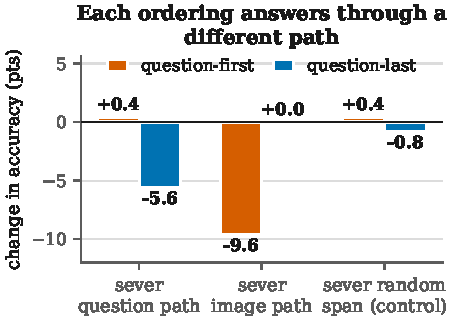
\includegraphics[width=0.52\textwidth]{figs/fig_knockout.pdf}
\end{center}
\caption{Each ordering answers through a different path. Bars are the change in
accuracy against the unmodified run ($57.6$ for question-first, $58.8$ for
question-last). Severing answer-to-question hurts only question-last; severing
answer-to-image hurts only question-first; the random span-size control moves
both by at most $0.8$ points.}
\label{fig:knockout}
\end{figure}

The paired bootstrap on the question-last question knockout gives
$\Delta = 0.056$ with a 95\% CI of $[+0.0199, +0.096]$, so the interval excludes
zero.

\section{Cross-model ladders in full}
\label{app:models}

\begin{table}[h]
\caption{NaturalBench ladder across five models ($1{,}900$ groups). Four of five
models lose accuracy when the question moves before the image. Missing entries
were not run. LLaVA-1.5's question-first group accuracy is exactly zero.}
\label{tab:models-nb}
\begin{center}
\small
\begin{tabular}{llrrrrr}
\toprule
Model & Metric & \sit{} & \sti{} & \stit{} & \sitit{} & $\Delta$ (\sti{}$-$\sit{}) \\
\midrule
Qwen3-VL-8B   & pair acc.  & 79.21 & 75.29 & 78.95 & \best{80.36} & $-3.92$ \\
              & group acc. & 35.05 & 26.95 & 35.00 & \best{37.37} & $-8.10$ \\
Qwen2.5-VL-7B & pair acc.  & \best{76.05} & 64.95 & 71.83 & 75.71 & $-11.10$ \\
              & group acc. & \best{27.74} & 10.16 & 19.11 & 27.63 & $-17.58$ \\
InternVL3-8B  & pair acc.  & 79.63 & 75.61 & 79.76 & \best{80.80} & $-4.02$ \\
              & group acc. & 35.53 & 27.63 & 36.47 & \best{39.32} & $-7.90$ \\
LLaVA-1.5     & pair acc.  & \best{66.87} & 50.26 & 66.29 & n/a & $-16.61$ \\
              & group acc. & \best{12.32} & 0.00 & 12.05 & n/a & $-12.32$ \\
Gemma-3-27B   & pair acc.  & 73.34 & 73.21 & \best{74.64} & 74.61 & $-0.13$ \\
              & group acc. & 22.63 & 23.21 & 25.26 & \best{25.53} & $+0.58$ \\
\bottomrule
\end{tabular}
\end{center}
\end{table}

\begin{table}[h]
\caption{Cross-model check on the four benchmarks run for all three models. The
question-first paradox does not replicate on either Gemma model, yet image
echoing is still the best ordering on 7 of 8 model-benchmark pairs.}
\label{tab:crossmodel}
\begin{center}
\small
\begin{tabular}{llrrrrrrr}
\toprule
 & & & \multicolumn{4}{c}{Ordering} & \multicolumn{2}{c}{$\Delta$ vs \sit{}} \\
\cmidrule(lr){4-7}\cmidrule(lr){8-9}
Model & Benchmark & $N$ & \sit{} & \sti{} & \stit{} & \sitit{} & \sti{} & \sitit{} \\
\midrule
\multirow{4}{*}{Gemma-3-27B}
 & BLINK   &     793 & 44.51 & 43.51 & 42.75 & \best{44.89} & $-1.01$ & $+0.38$ \\
 & MMVP    &     300 & 72.67 & 72.33 & 72.00 & \best{74.67} & $-0.33$ & $+2.00$ \\
 & TallyQA &  38{,}589 & 63.00 & 67.60 & 68.93 & \best{69.97} & $+4.60$ & $+6.96$ \\
 & VQAv2   & 214{,}354 & \best{64.77} & 62.07 & 63.04 & 62.07 & $-2.70$ & $-2.70$ \\
\cmidrule(lr){2-9}
 & \emph{Mean} & & & & & & $+0.14$ & $+1.66$ \\
\midrule
\multirow{4}{*}{Gemma-4-31B}
 & BLINK   &     793 & 54.48 & 56.12 & 56.12 & \best{56.49} & $+1.64$ & $+2.02$ \\
 & MMVP    &     300 & 84.67 & 86.00 & 86.67 & \best{87.33} & $+1.33$ & $+2.67$ \\
 & TallyQA &   2{,}000 & 80.65 & 80.50 & 81.20 & \best{82.60} & $-0.15$ & $+1.95$ \\
 & VQAv2   &   3{,}000 & 73.50 & 74.66 & 75.65 & \best{76.00} & $+1.16$ & $+2.50$ \\
\cmidrule(lr){2-9}
 & \emph{Mean} & & & & & & $+1.00$ & $+2.28$ \\
\bottomrule
\end{tabular}
\end{center}
\end{table}

\section{Significance tests in full}
\label{app:significance}

Paired on group index (NaturalBench) or example index (Winoground), exact
two-sided McNemar plus a paired bootstrap 95\% CI over $5{,}000$ resamples,
seed 0. Accuracies are group accuracy.

\begin{table}[h]
\caption{Significance for consecutive rungs of the ladder and for the headline
comparisons. \sti{} versus \sit{} is highly significant for Qwen3-VL-8B on both
benchmarks and absent for Gemma-3-27B. \sitit{} versus \sit{} is significant on
Winoground for both models.}
\label{tab:significance}
\begin{center}
\scriptsize
\setlength{\tabcolsep}{3pt}
\begin{tabular}{lllrrrl}
\toprule
Benchmark & Model & Comparison & acc A & acc B & $\Delta$ (95\% CI) & McNemar $p$ \\
\midrule
NaturalBench & Qwen3-VL-8B & \sti{} vs \sit{}   & 0.269 & 0.351 & $+0.081$ $[+0.058, +0.103]$ & $1.3\times10^{-12}$ \\
             &             & \sit{} vs \stit{}  & 0.351 & 0.350 & $-0.001$ $[-0.022, +0.020]$ & $1.00$ \\
             &             & \stit{} vs \sitit{} & 0.350 & 0.374 & $+0.024$ $[+0.005, +0.043]$ & $1.6\times10^{-2}$ \\
             &             & \sitit{} vs \sititrev{} & 0.374 & 0.374 & $+0.000$ $[-0.010, +0.011]$ & $1.00$ \\
\cmidrule(lr){2-7}
             & Gemma-3-27B & \sti{} vs \sit{}   & 0.232 & 0.226 & $-0.006$ $[-0.026, +0.015]$ & $0.62$ \\
             &             & \sit{} vs \stit{}  & 0.226 & 0.253 & $+0.026$ $[+0.006, +0.046]$ & $1.4\times10^{-2}$ \\
             &             & \stit{} vs \sitit{} & 0.253 & 0.255 & $+0.003$ $[-0.015, +0.021]$ & $0.82$ \\
\midrule
Winoground   & Qwen3-VL-8B & \sti{} vs \sit{}   & 0.223 & 0.318 & $+0.095$ $[+0.050, +0.140]$ & $7.7\times10^{-5}$ \\
             &             & \sit{} vs \stit{}  & 0.318 & 0.375 & $+0.057$ $[+0.015, +0.102]$ & $1.2\times10^{-2}$ \\
             &             & \sit{} vs \sitit{} & 0.318 & 0.403 & $+0.085$ $[+0.045, +0.125]$ & $2.4\times10^{-5}$ \\
             &             & \sti{} vs \sititrev{} & 0.223 & 0.410 & $+0.187$ $[+0.140, +0.235]$ & $1.2\times10^{-13}$ \\
\cmidrule(lr){2-7}
             & Gemma-3-27B & \sti{} vs \sit{}   & 0.212 & 0.207 & $-0.005$ $[-0.052, +0.043]$ & $0.92$ \\
             &             & \sit{} vs \stit{}  & 0.207 & 0.253 & $+0.045$ $[+0.000, +0.087]$ & $6.3\times10^{-2}$ \\
             &             & \sit{} vs \sitit{} & 0.207 & 0.318 & $+0.110$ $[+0.070, +0.152]$ & $8.1\times10^{-7}$ \\
\bottomrule
\end{tabular}
\end{center}
\end{table}

\section{Read-out probe and decision layer in full}
\label{app:probe}

Qwen3-VL-8B, 36 layers. The disagreement set is the $150$ NaturalBench pairs
where \sti{} is wrong and \sit{} is right; the decision-layer analysis uses
$300$ pairs. $a_q$ and $a_{img}$ are attention mass from the answer position onto
the question and image spans, averaged over heads.

\begin{table}[h]
\caption{Read-out probe on the disagreement set. \sti{} peaks lower on the
question and much higher on the image, and the mid-to-late band ratio inverts.}
\label{tab:probe}
\begin{center}
\begin{tabular}{lrrrrr}
\toprule
Ordering & probe acc & $\max a_q$ (layer) & $\max a_{img}$ (layer) & $a_q{:}a_{img}$ @L24 & final $P(\text{gt})$ \\
\midrule
\sti{}      & 0.073 & 0.0676 (23) & 0.2367 (21) & 0.424 & 0.1346 \\
\sit{}      & 0.887 & 0.1479 (23) & 0.0942 (18) & 1.065 & 0.8485 \\
\stit{}     & 0.600 & 0.1437 (23) & 0.1448 (21) & 0.986 & 0.5912 \\
\sitit{}    & 0.847 & 0.1286 (23) & 0.0647 (26) & 1.544 & 0.8374 \\
\sititrev{} & 0.867 & 0.1218 (23) & 0.0617 (26) & 1.624 & 0.8503 \\
\bottomrule
\end{tabular}
\end{center}
\end{table}

$P(\text{correct})$ over the $\{$Yes, No$\}$ decision on the $300$-pair
disagreement set. All four orderings sit at $\approx 0.50$ through layer 25, so
only layers 26 to 35 are shown.

\begin{center}
\footnotesize
\setlength{\tabcolsep}{3.5pt}
\begin{tabular}{lrrrrrrrrrr}
\toprule
Layer & 26 & 27 & 28 & 29 & 30 & 31 & 32 & 33 & 34 & 35 \\
\midrule
\sti{}   & 0.480 & 0.456 & 0.440 & 0.449 & 0.495 & 0.429 & 0.398 & 0.222 & 0.099 & 0.152 \\
\sit{}   & 0.593 & 0.665 & 0.680 & 0.663 & 0.529 & 0.691 & 0.728 & 0.824 & 0.875 & 0.851 \\
\sitit{} & 0.624 & 0.691 & 0.710 & 0.704 & 0.546 & 0.704 & 0.722 & 0.827 & 0.819 & 0.827 \\
\stit{}  & 0.526 & 0.513 & 0.523 & 0.521 & 0.500 & 0.532 & 0.533 & 0.547 & 0.553 & 0.570 \\
\bottomrule
\end{tabular}
\end{center}

\section{Per-patch cosine to an image-only forward pass}
\label{app:cosine}

Layer 18, images resized to $448\times448$, $14\times14 = 196$ patches,
Qwen3-VL-8B. Mean per-patch cosine between each ordering's image-token hidden
states and a forward pass on the image alone.

\begin{table}[h]
\caption{The question rewrites the image tokens. \ist{} is the image-only
baseline by construction; \stit{} is identical to \sti{} because causal masking
prevents a later question copy from affecting earlier patches.}
\label{tab:cosine}
\begin{center}
\begin{tabular}{lrrrr}
\toprule
Ordering & $n$ & mean cos & median & min \\
\midrule
\ist{}  & 7{,}600 & 0.999998 & 1.000000 & 0.999919 \\
\sit{}  & 30 & 0.911017 & 0.921399 & 0.722478 \\
\sti{}  & 7{,}600 & 0.862723 & 0.873233 & 0.614870 \\
\stit{} & 7{,}600 & 0.862727 & 0.873237 & 0.614835 \\
\bottomrule
\end{tabular}
\end{center}
\end{table}

Sanity checks: $\cos(\text{base}, \ist{}) = 0.999997$ and
$\cos(\sti{}, \stit{}) = 0.999992$ at $n = 7{,}600$.

\section{Exact token cost per ordering}
\label{app:cost}

\begin{table}[h]
\caption{Exact token cost per query, mean over 20 images spanning RF20's
constituent datasets, Qwen3-VL-8B. $\Delta$ is against the \sti{} baseline.
\sti{} and \sit{} contain the same tokens in a different order, so their totals
are identical. Repeating the question is nearly free; repeating the image is not,
but its cost falls with echo area because vision tokens scale with pixels.}
\label{tab:cost}
\begin{center}
\begin{tabular}{lrrrrrr}
\toprule
Prompt & Total & Image & Text & $\Delta$ total & $\Delta$ image & $\Delta$ text \\
\midrule
\sti{} (baseline)            & 3385.8 & 3335.8 & 50.0 & n/a & n/a & n/a \\
\stit{} (question echo)      & 3398.8 & 3335.8 & 63.0 & $+13.0$ & $+0.0$ & $+13.0$ \\
\sitit{}, echo $1$           & 6737.5 & 6671.5 & 66.0 & $+3351.8$ & $+3335.8$ & $+16.0$ \\
\sitit{}, echo $\tfrac{1}{2}$ & 4260.7 & 4194.7 & 66.0 & $+874.9$ & $+858.9$ & $+16.0$ \\
\sitit{}, echo $\tfrac{1}{4}$ & 3637.6 & 3571.6 & 66.0 & $+251.8$ & $+235.8$ & $+16.0$ \\
\sitit{}, echo $\tfrac{1}{8}$ & 3492.6 & 3426.6 & 66.0 & $+106.8$ & $+90.8$ & $+16.0$ \\
\bottomrule
\end{tabular}
\end{center}
\end{table}

\section{GEPA configuration and training cost}
\label{app:gepa}


GEPA \citep{gepa2025} optimizes the system message only. The task model is
Qwen3-VL-8B; the reflection model is Gemma-3-27B on a separate GPU, since
reusing the task model as its own reflector produced proposals that never passed
GEPA's strict-improvement acceptance test. Training and validation examples are
disjoint from the held-out evaluation set.

\begin{table}[h]
\caption{GEPA search budget and cost, \sti{} ordering. Training tokens are a
one-time cost; the per-query cost is the prompt-length delta in
Table~\ref{tab:gepa-tokens}.}
\label{tab:gepa-cost}
\begin{center}
\begin{tabular}{lrrrrr}
\toprule
Benchmark & train & val & metric calls & training tokens & wall clock (s) \\
\midrule
POPE         & 100 & 60 & 400 & 157{,}725 & 124.3 \\
VQAv2        & 150 & 80 & 1{,}008 & 396{,}253 & 232.4 \\
NaturalBench & 250 & 120 & 1{,}540 & 982{,}343 & 528.7 \\
\bottomrule
\end{tabular}
\end{center}
\end{table}

\begin{table}[h]
\caption{Prompt-length cost of GEPA's optimized system messages, in tokens per
query. Under \sit{} on POPE and VQAv2 the optimizer returned the seed prompt, so
the delta is zero.}
\label{tab:gepa-tokens}
\begin{center}
\begin{tabular}{llrrr}
\toprule
Benchmark & Order & seed & optimized & $\Delta$ \\
\midrule
POPE         & \sti{} & 315 & 341 & $+26$ \\
             & \sit{} & 316 & 316 & $+0$ \\
VQAv2        & \sti{} & 313 & 345 & $+32$ \\
             & \sit{} & 314 & 314 & $+0$ \\
NaturalBench & \sti{} & 216 & 287 & $+71$ \\
             & \sit{} & 217 & 381 & $+164$ \\
\bottomrule
\end{tabular}
\end{center}
\end{table}

\section{Logit-lens word divergence between \sti{} and \ist{}}
\label{app:worddiff}

To ask whether question-first and image-first prompting diverge in the words they
are internally predicting, we decode the top-1 token at every (layer, generation
step) position under both orderings on 100 samples, discard positions whose two
words are identical or WordNet synonyms, and discard any position where either
side is not a dictionary word, since intermediate layers frequently project onto
subword fragments.

Genuine word changes are rare and concentrated: $8$ across 100 samples, of which
$6$ occur at layer 16, one at layer 8 and one at layer 20, with none at layers
0, 4, 12, 24 or 27. Divergence at the level of decoded output words is therefore
sparse and mid-network, consistent with the read-out account in
Section~\ref{sec:background-readout}, where the two orderings are indistinguishable
at the decision level until late and differ mainly in routing rather than in
vocabulary.

\section{Reproduction notes}
\label{app:repro}

Every accuracy in this paper is read from a per-run result file that records the
model, the ordering, the system prompt, the decoding budget and the sample count.
Two details are worth flagging for anyone re-running the analysis.

The attention knockout must restrict the query side to the answer position. With
the query side widened to every position after the question, the question-side
half of the dissociation does not reproduce (severing answer-to-question raises
\sit{} by $2.8$ points, CI $[-0.084, +0.028]$), and the random-span control is
itself worth $10$ points on \sti{}, so that configuration is uninformative rather
than contradictory.

The Gemma-3-27B RF20 run is degenerate and we exclude it from all RF20 claims.
It answers ``yes'' to roughly $96\%$ of items under every ordering
(\texttt{yes\_ratio} $0.955$ to $0.964$, recall $0.979$ to $0.991$), so its
accuracy sits at the positive base rate and the spread across orderings is
$0.003$.
